\chapter{Method Selection and Planning}
\section{Outline and Justification of Software Engineering Methods and Tools}

Choosing a set of software engineering methods for our SEPR project has required careful consideration from us as a team.
Many factors can influence the suitability of certain methods for a project, such as team size, the type of system being delivered and the volatility of user requirements.
It was through the analysis of these type of factors that we came to a decision about which methods we would be using.

A key aspect of a software engineering method is its development lifecycle, which dictates and characterises each engineering activity.
Many different lifecycles exist, with varying characteristics, so it was important for us to explore some different types and decide which one was best for our project.
We decided that methods based on an incremental development lifecycle would be most suited to us, as it protects us against volatile requirements and allows us to regularly get feedback from our customer.
This means we can produce an end result which is as close to our customers expectations as possible. We explored alternative lifecycles to the incremental approach, including the “waterfall” approach proposed by Winston Royce~\cite{royce1970managing}.
We discarded this approach however because the model struggles to deal with changes of requirements, and also has large documentation overheads which are not necessary for the size of our project.
There is also risk involved with this model as the first time the customer sees the software is at the end of the lifecycle, so if they are not satisfied then it will be very hard to fix broken procedures and implement new ones.

Now that we had decided on our development lifecycle, we next had to decide on a set of engineering methods and principles which fit the incremental approach.
Once again, there are a large number of methods which fit this approach so an investigation of these methods and their differences was required.

We looked at the Rational Unified Process (RUP) proposed by Rational, now a division of IBM, which is a plan-based incremental engineering method.
RUP splits each iteration of the development lifecycle into four phases, called the inception phase, elaboration phase, construction phase and transition phase.
Each phase has a well defined milestone which is achieved at the end of the phase~\cite{rup1998}.
The first two phases involve the creation of a requirements list, use cases, risk assessments, project plans, a system architecture amongst other planning phase documents.
The next two phases are all about the development, testing and integration of the system into the customer’s working environment.
After evaluation and consideration, we decided that RUP wouldn’t be best suited to our project.
The problem we found was that in order to use this development process, you need strong knowledge from the outset of how the system will work in order to develop the use cases.
While we have been given a brief, from interviewing our customer we discovered that certain features have been left up to us to develop, meaning that working through the first two phases of RUP in each lifecycle would be difficult and cost us time, leaving us with less time to actually develop the software.
Also, according to Boehm, “only change rates on the order of 1\% of the requirements are acceptable” for plan-based development~\cite[p 31]{boehm2003balancing}.
With our project, requirements may change on a regular basis, meaning that this approach may not be able to cope.

We decided instead to adopt an Agile approach to the software engineering of this project due to its merging of design and implementation phases and short iteration lifecycles which will allow the system to organically grow as we incorporate customer feedback into the development process. We will mainly be following the eXtreme Programming (XP) and Scrum agile methods, as the principles in each method work very well for small teams who can stay in regular contact with their customer, which is perfect for us. Some of the principles from the eXtreme Programming agile method that we will be using in the development of our project are:
\begin{itemize}
	\item Test Driven Development (TDD)
	\item Refactoring
	\item Incremental Planning \& User Stories
	\item Pair Programming
	\item Small releases \& updates of the final product~\cite{sommerville2016software}
\end{itemize}

In order to write code and collaborate as a team, we are going to need a version control system.
Git seems like a suitable option, as it allows us to work on different sections of code together in local repositories before committing updates to the main repository without blocking each other's productivity.
A good team also requires good communication, so we will be using the Slack service as it allows us to talk on multiple channels, and integrate other services into conversations (e.g. Git commits and updates).
Organising tasks which need to be completed is another important part of collaboration, and Trello provides a very nice way of doing this.
We can set up different “cards” on a Trello dashboard for different backlogs of task, meaning that we always know what needs to be completed, what is being completed and what has been completed.

\section{Team Organisation}

Team organisation can be the difference between a successful project and a failure, so we took the time to choose an approach to organisation which will allow the team to collaborate effectively, and reflect on improvements we need to make as a team in order to be successful.
The Scrum methodology seems like an excellent way to organise the team, and fits in well with the other Agile methods and principles we are using e.g. user stories from eXtreme Programming~\cite{sommerville2016software}.

We will begin each iteration of our software lifecycle by reviewing our current user stories and breaking them down into tasks which can then be implemented into the system.
Test cases can also be generated from these stories for Test Driven Development.
We will have a Trello dashboard with cards for the Product Backlog and the Sprint Backlog where all the tasks and the current sprint tasks respectively will be stored, allowing us to move tasks from the left to the right as they are completed by the team.
Once the tasks we are completing during the sprint have been established, we will carry out the sprint which will last for around 4 - 5 days.
During this time we will attempt to implement as many of the tasks in the Sprint Backlog as we can, as well as having a regular meeting each day called a Scrum where we say what we are working on, how we are getting on with it, and if we are having any issues.
After the sprint is finished, we should ideally have a version of our system that is working and includes all of the functionality we have implemented so far.
We will then have a sprint review, where we discuss how the sprint went, if there is any outstanding functionality which wasn't implemented during the sprint and if there are any ways in which we can improve team productivity. 

\begin{landscape}
	\section{Project Plan}
	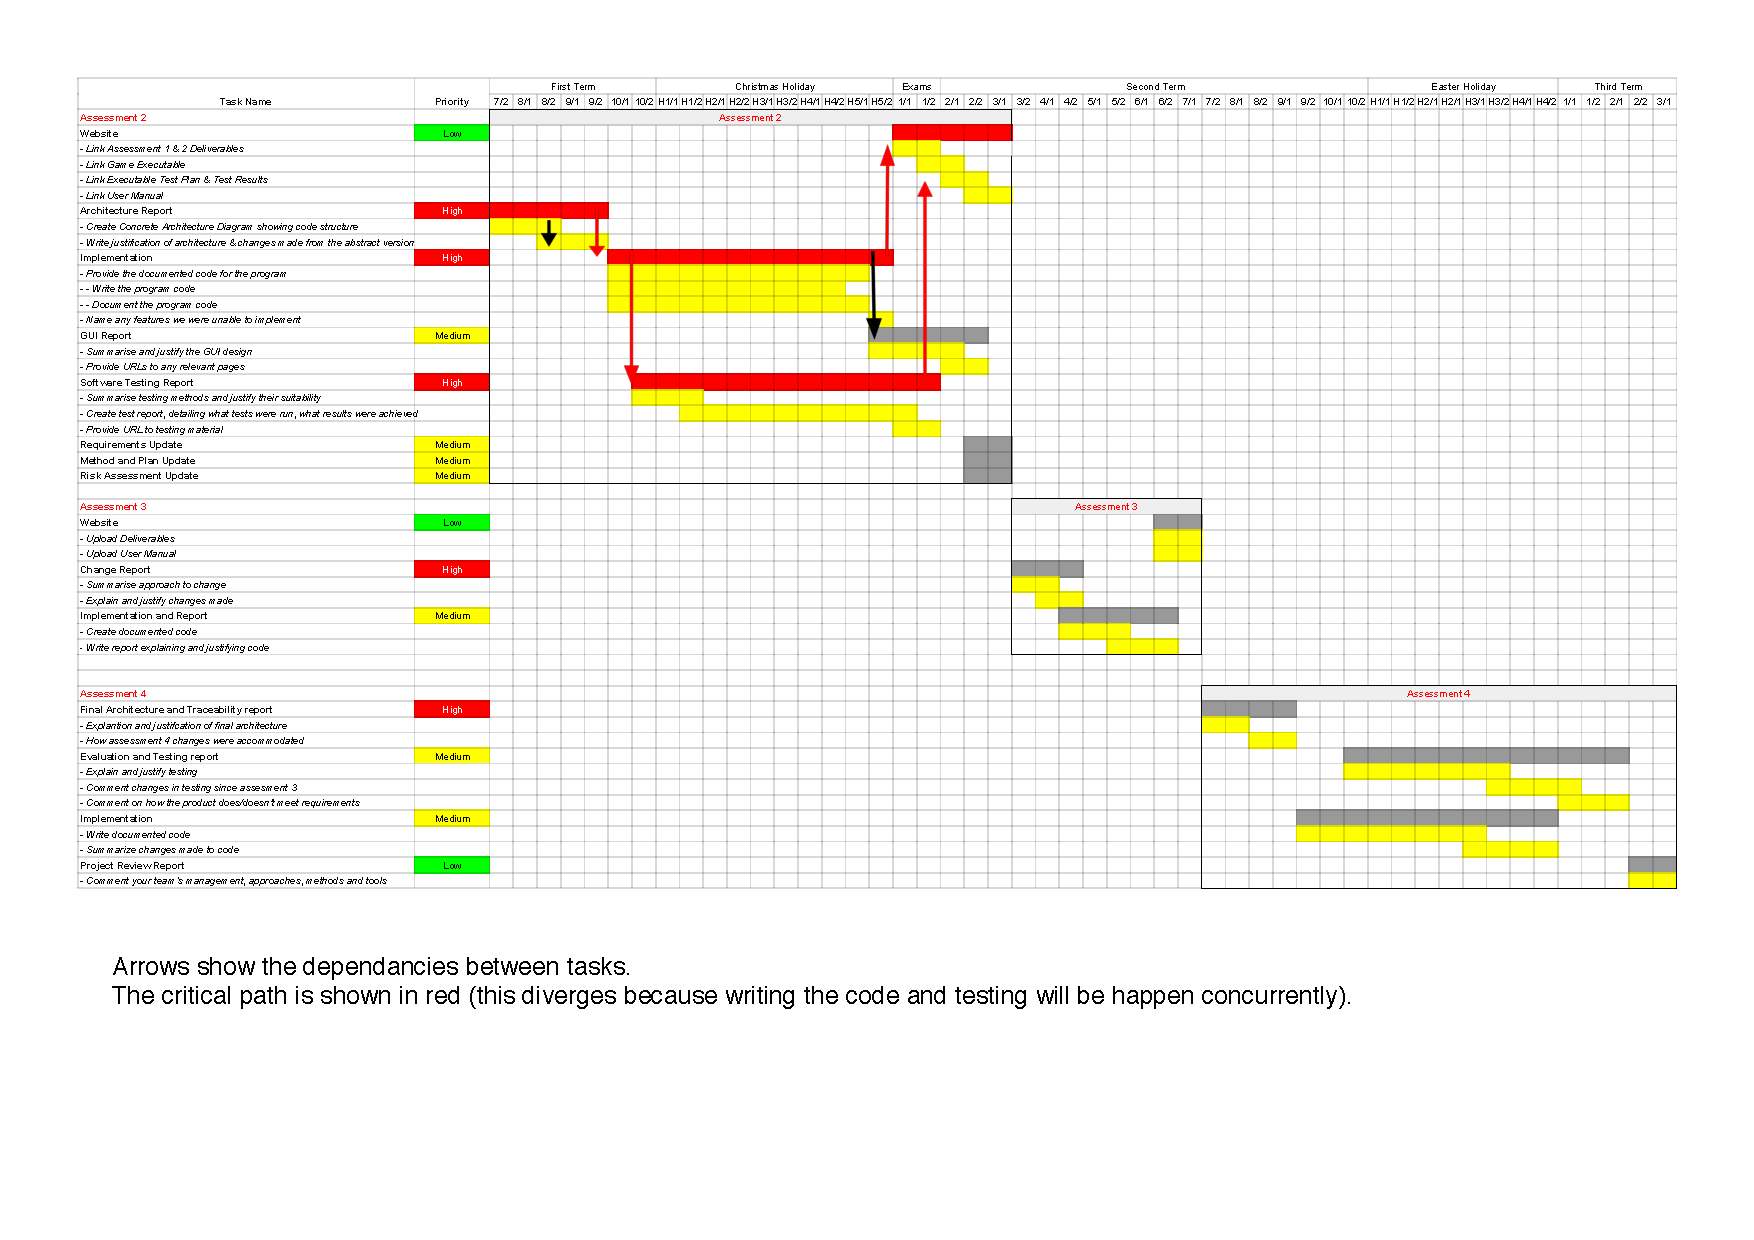
\includegraphics[width=9.85in]{plan.pdf}
\end{landscape}

\bibliographystyle{ieeetr}
\bibliography{references.bib}